\documentclass[preprint,12pt]{elsarticle}


%% The `ecrc' package must be called to make the CRC functionality available
%\usepackage{ecrc}

%% set the volume if you know. Otherwise `00'
%\volume{00}

%% set the starting page if not 1
%\firstpage{1}

%% Give the name of the journal
%\journalname{Expert Systems With Applications}

%% Give the author list to appear in the running head
%% Example \runauth{C.V. Radhakrishnan et al.}
%\runauth{}

%% The choice of journal logo is determined by the \jid and \jnltitlelogo commands.
%% A user-supplied logo with the name <\jid>logo.pdf will be inserted if present.
%% e.g. if \jid{yspmi} the system will look for a file yspmilogo.pdf
%% Otherwise the content of \jnltitlelogo will be set between horizontal lines as a default logo

%% Give the abbreviation of the Journal.  Contact the journal editorial office if in any doubt
%\jid{eswa}

%% Give a short journal name for the dummy logo (if needed)
%\jnltitlelogo{ESWA Logo}

%% Provide the copyright line to appear in the abstract
%% Usage:
%   \CopyrightLine[<text-before-year>]{<year>}{<restt-of-the-copyright-text>}
%   \CopyrightLine[Crown copyright]{2011}{Published by Elsevier Ltd.}
%   \CopyrightLine{2011}{Elsevier Ltd. All rights reserved}
%\CopyrightLine{2013}{Published by Elsevier Ltd.}



%\usepackage{llncsdoc}
\usepackage[figuresright]{rotating}
%\usepackage{makeidx}  % allows for indexgeneration
\usepackage{graphicx}
\usepackage[T1]{fontenc}
\usepackage[english]{babel}
\usepackage[utf8]{inputenc}
\usepackage{multirow}

\usepackage{url}
\usepackage{rotating}

%%%Math
\usepackage{latexsym}
 \usepackage{amsmath}
% \usepackage{amssymb}
% \usepackage{amsthm}
%\usepackage{eurosans}

\usepackage{eurosym}

\usepackage{longtable}

\usepackage{listings}

\usepackage{color}
\usepackage{textcomp}


\definecolor{gray}{gray}{0.5}
\definecolor{green}{rgb}{0,0.5,0}
% 
% \usepackage{inconsolata}



\begin{document}


\begin{frontmatter}

%% Title, authors and addresses

%% use the tnoteref command within \title for footnotes;
%% use the tnotetext command for the associated footnote;
%% use the fnref command within \author or \address for footnotes;
%% use the fntext command for the associated footnote;
%% use the corref command within \author for corresponding author footnotes;
%% use the cortext command for the associated footnote;
%% use the ead command for the email address,
%% and the form \ead[url] for the home page:
%%
%% \title{Title\tnoteref{label1}}
%% \tnotetext[label1]{}
%% \author{Name\corref{cor1}\fnref{label2}}
%% \ead{email address}
%% \ead[url]{home page}
%% \fntext[label2]{}
%% \cortext[cor1]{}
%% \address{Address\fnref{label3}}
%% \fntext[label3]{}

%\dochead{}
%% Use \dochead if there is an article header, e.g. \dochead{Short communication}
%% \dochead can also be used to include a conference title, if directed by the editors
%% e.g. \dochead{17th International Conference on Dynamical Processes in Excited States of Solids}


\title{Empowering the access to public procurement opportunities by means of linking controlled vocabularies.  A case study of Product Scheme Classifications in the European e-Procurement sector.}


%% use optional labels to link authors explicitly to addresses:
\author[label1]{Jose María Alvarez-Rodríguez\corref{cor1}}
\address[label1]{The South East European Research Center, Thessaloniki, Greece.}
\ead{jmalvarez@seerc.org}
\ead[url]{http://www.seerc.org}

\author[label2]{José Emilio Labra-Gayo}
\address[label2]{WESO Research Group, Department of Computer Science, University of Oviedo, 33007, Oviedo, Spain.}
\ead{labra@uniovi.es}

\author[label3]{Alejandro Rodríguez-González}
\address[label3]{Bioinformatics at Centre for Plant Biotechnology and Genomics UPM-INIA, Polytechnic University of Madrid, Madrid, Spain.}
\ead{alejandro.rodriguezg@upm.es}

\author[label4]{Patricia Ordoñez De Pablos}
\address[label4]{WESO Research Group, Department of Business Administration, University of Oviedo, 33007, Oviedo, Spain.}
\ead{patriop@uniovi.es}





\author{}

\address{}

\begin{abstract}
The present paper introduces a method to promote existing controlled vocabularies to 
the Linked Data initiative. A common data model and an enclosed conversion 
method for knowledge organization systems based on semantic web technologies and 
vocabularies such as SKOS are presented. This method is applied to well-known 
taxonomies and controlled vocabularies in the business sector, more specifically 
to Product Scheme Classifications created by governmental institutions such as 
the European Union or the United Nations. Since these product schemes are 
available in a common and shared data model, the needs of the European 
e-Procurement sector are outlined to finally demonstrate how Linked Data can 
address some of the challenges for publishing and retrieving information 
resources. As a consequence, two experiments are also provided in order to 
validate the gain, in terms of expressivity, and the exploitation of this emerging 
approach to help both expert and end-users to make decisions on the selection of descriptors 
for public procurement notices.
\end{abstract}

\begin{keyword}
%% keywords here, in the form: keyword \sep keyword
e-Procurement \sep product scheme classifications \sep  linked open data \sep  semantic web \sep expert systems
%% PACS codes here, in the form: \PACS code \sep code

%% MSC codes here, in the form: \MSC code \sep code
%% or \MSC[2008] code \sep code (2000 is the default)

\end{keyword}


\end{frontmatter}

\section{Introduction}
Government bodies and public institutions as a whole are the most important buyers in the European Union (EU), since public procurement spending represents around 19\% of 
EU Gross Domestic Product (GDP)~\cite{d2010}. Given this situation there is a growing interest and commitment~\cite{d2010a} to ensure that these funds are 
well managed and most of inefficiencies are eliminated. Electronic public procurement or e-Procurement~\cite{Podlogar2007} emerges as an alternative to link and 
integrate inter-organizational business processes and systems with the automation of the requisitioning, the approval purchase order 
management, accounting processes among others through the Internet-based protocol. However there is much more at stake than the mere changeover 
from paper based systems to ones using electronic communications. It should have the potential to yield important improvements in the access to information and data such as the efficiency of individual purchases, 
the overall administration of public procurement or the functioning of the markets for government contracts. 

In this context the European Commission (EC) is trying to unlock this potential, the 2004 Public Procurement Directives 2004/17/EC and 2004/18/EC 
introduced several provisions and projects~\cite{peppol,e-certis} aimed at enabling e-Procurement uptake in all Member States. In this light of 
modernizing the European public procurement sector to support growth and employment the EC also identified~\cite{siemensEval} 
both regulatory and natural barriers in the access to public procurement in the EU context, especially for SMEs. 
According to this evaluation, a real European Single Market use~\cite{d2011} has not yet been achieved causing losses, 
being cost-inefficient, missing opportunities for society and leading to a situation where more than 27 national markets co-exist instead of an EU-wide public market~\cite{monti2010}. 
In this sense, one relevant action to ease the interconnectivity and interoperability in this landscape was the creation of the Tenders Electronic Daily~\cite{eNotices,formsTed} (TED) 
by the EC. It is the on-line version of the ``Supplement to the Official Journal of the European Union'', dedicated to European public procurement notices 
($1500$ new announcements every day) but a unified pan-European information system dealing with: dispersion of the information, 
duplication of the same notice in more than one source, different publishing formats, problems with regards to a multilingual environment and 
aggregation of low-value procurement opportunities, is still missing. As a consequence some of the potential advantages 
outlined by the EC~\cite{d2010} such as increased accessibility and transparency, benefits for individual procedures, 
benefits in terms of more efficient procurement administration and potential for integration of EU procurement markets cannot be reached in a 
short-term.

Furthermore other EU actions in the e-Government context have been focused on the development of conceptual/terminological maps available in the Eurostat's metadata server (RAMON): 
in the Health field, the ``European Schedule of Occupational Diseases'' or  the ``International Classification of Diseases''; in the Education field,  
thesauri as the ``European Education Thesaurus''; in the Employment field, the ``International Standard Classification of Occupations''; 
in the European Parliament activities the ``Eurovoc Thesaurus'' and in the e-Procurement field the ``Common Procurement Vocabulary'' (CPV). 
The structure and features of these systems are very heterogeneous, although some common aspects can be found in all of them: hierarchical relationships between terms or concepts and multilingual character of the information. 
These knowledge organization systems (KOS) enable users to annotate information objects providing an agile mechanism for performing 
tasks such as exploration, searching, automatic classification or reasoning. Nevertheless depending on the country and the scope 
distinct classifications are commonly used. In the specific case of e-Procurement, the United Nations Standard Products and Services Code (UNSPSC) in Australia, 
the North American Industry Classification System (NAICS) in United States or the CPV and TARIC (Integrated Tariff of the European Communities) in the European Union 
are examples of similar efforts to unify and model procurement-related data. As a consequence a real, standardized and integrated environment 
for e-Procurement (and business) data to encourage the creation of knowledge-based services cannot be easily deployed. In this sense the 
``European Code of Best Practices Facilitating Access by SMEs to Public Procurement Contracts''~\cite{d2008} pointed out 
two groups of difficulties regarding the barriers faced by SMEs in accessing relevant information about public procurement opportunities. 
The document stated that ``the (big) number of such web portals being used by the government and by regional and local authorities makes it difficult 
for tenderers to maintain an overview''. By aggregating data on public procurement in all Member States 
and at all administrative levels in a standardized way and reusing existing efforts of modeling 
and classifying domain knowledge, some open and critical issues can be tackled to improve a situation which affects more 
than \euro $20$ million non-financial companies established in the EU.


On the other hand and following the principles of the Open Data initiative, the vice-president Neelie Kroes is leading the Open Data Strategy for Europe. 
She also outlined in December 2011 several types of actions that will help to unleash potential of data held by governments in Europe. The strategy is 
strongly focused on the commercial value of the re-use of Public Sector Information (PSI), by which the Commission expects to deliver a \euro 40 billion boost to the EU's economy each year. 
A new version of the 2003 Public Sector Information Directive~\cite{d2003} is also expected and the EC is strongly determined to act as a global leader along with United States, 
Canada or Australia. This open data is supposed to enable greater transparency; delivers more efficient public services; and encourages greater 
public and commercial use. More specifically in the context of e-Procurement the access to public contracts announcements is the first natural 
step to encourage SME participation and create a real public market of procurement opportunities.


Moreover, the emerging Web of Data and the sheer mass of information now available make it possible the deployment of new 
added-value services and applications based on the reuse of existing vocabularies and datasets. 
The popular diagram of the Linked Data Cloud~\cite{linked-data-cloud}, generated from metadata extracted from the 
Comprehensive Knowledge Archive Network (CKAN) out, contains $336$ datasets, with more than 25 billion RDF triples and 395 million links. 
With regards to e-Procurement, a new group of 130 CKAN datasets have been released from the ``OpenSpending.org'' site. In this realm, 
data coming from different sources and domains have been promoted following the principles of the 
Linked Data initiative~\cite{Berners-Lee-2006} to improve the access to large documental databases, 
e.g. e-Government resources, scientific publications or e-Health records. In the case of KOS, such as thesauri, taxonomies or classification systems 
are developed by specific communities and institutions in order to organize huge collections of information objects. 
These vocabularies allow users to annotate~\cite{Leukel-standard,Leukel-automating,Leukel-comparative} the information objects and easily retrieve them, 
promoting lightweight reasoning in the Semantic Web. Topic or subject indexing is an easy way to introduce machine-readable metadata for a resource's content 
description. Indeed, Product Scheme Classifications (also known as PSCs), such as the CPV, are a kind of KOS that have been built to solve specific problems 
of interoperability and communication between e-Commerce agents~\cite{FenselOmel2001,Leukel-findings}, in the particular case of PSCs they are considered to be a key-enabler of 
the next European e-Procurement domain and other supply chain processes~\cite{DBLP:journals/tcci/Alor-HernandezAJPRMBG10}.

Obviously the public information published by governmental contracting authorities, more specifically PSCs, are a suitable candidate to apply the Linked (Open) Data 
(LOD) principles and semantic web technologies providing a new environment in which the conjunction of these initiatives can provide the building blocks for an 
innovative unified pan-European information system that encourages standardization of key processes and systems and gives economic operators the tools to overcome 
technical interoperability easing and enhancing the access and reuse of public information. Therefore main contributions of this paper lay in:
\begin{itemize}
\item Modeling, transforming and interlinking the structure and data of PSCs developed by public bodies following the LOD principles.
\item Publishing all information via an SPARQL endpoint providing a public procurement Linked Data node and, more specifically, a new PSCs catalogue as Linked Data.
\item Exploiting the aforementioned catalogue via a contract descriptor recommendation service.
\item Demonstrating the gain (in terms of number of descriptors to retrieve public procurement notices) and the semantic exploitation 
capabilities of the new PSCs catalogue.
\end{itemize}

The remainder of this paper is structured as follows. Section~\ref{sect:related-work} reviews the relevant literature. Next thesauri 
conversion methods are outlined. Section~\ref{sect:method} presents the application of a method for promoting raw data to the LOD initiative 
and its application to the PSCs in the European e-Procurement sector. Section~\ref{sect:evaluation} describes the evaluation of applying the LOD principles to 
these product schemes through two studies that include a description of the sample, the method, results and discussion. Finally, 
the paper ends with a discussion of research findings, limitations and some concluding remarks.

\section{Literature Review}\label{sect:related-work}
According to the previous section, some relevant works can be found and grouped by the topics covered in this paper:

\begin{itemize}
 \item  The Semantic Web area, coined by Tim Berners-Lee in 2001, has experienced during last years a growing 
 commitment from both academia and industrial areas  with the objective of elevating the meaning of web 
 information resources through a common and shared data model (graphs) and an underlying semantics based 
 on different logic formalisms (ontologies). The Resource Description Framework (RDF), based on a graph model, and the Web Ontology Language (OWL), designed to formalize and model domain knowledge, are the two main \textit{ingredients} to reuse information and data 
 in a knowledge-based realm. Thus data, information and knowledge can be easily shared, exchanged and linked~\cite{Maali_Cyganiak_2011} 
 to other knowledge and databases through the use URIs, more specifically HTTP-URIs. Therefore the broad objective of this effort can be summarized 
 as a new environment of added-value information and services that can encourage and improve B2B (Business to Business), B2C (Business to Client) or 
 A2A (Administration to Administration) relationships by means of the implementation of new contex-awareness expert systems to tackle existing 
 cross-domain problems such as medical reasoning, analysis of social media, etc. in which data heterogeneities, 
 lack of standard knowledge representation and interoperability problems are common factors. As a practical view of the Semantic Web, 
 the Linked Data~\cite{Berners-Lee-2006,Heath_Bizer_2011} initiative emerges to create a large and distributed database on the Web. 
 In order to reach this major objective the publication of information and data under a common data model (RDF) 
 with a specific formal query language (SPARQL~\cite{Sparql11}) provides the required building blocks to turn the Web of documents 
 into a real database or ``Web of Data''. Research works are focused in two main areas: 1) production/publishing~\cite{bizer07how} and 2) consumption of 
 Linked Data. In the first case data quality~\cite{bizer2007,wiqa,ld-quality,DBLP:journals/ws/BizerC09,lodq,link-qa}, conformance~\cite{DBLP:journals/ws/HoganUHCPD12}, 
 provenance~\cite{w3c-prov,DBLP:conf/ipaw/HartigZ10}, trust~\cite{Carroll05namedgraphs}, description of 
 datasets~\cite{void,Cyganiak08semanticsitemaps,ckanValidator} and entity reconciliation~\cite{Serimi,Maali_Cyganiak_2011} are 
 becoming major objectives since a mass of amount data is already available through RDF repositories and SPARQL endpoints. 
 
 On the other hand, consumption of Linked Data is being addressed to provide new ways of data 
 visualization~\cite{DBLP:journals/semweb/DadzieR11,hoga-etal-2011-swse-JWS}, faceted browsing~\cite{Pietriga06fresnel, citeulike:8529753,Sparallax}, 
 searching~\cite{hoga-etal-2011-swse-JWS} and data exploitation~\cite{Harth:2011:SIP:1963192.1963318}. Some approaches 
 based on sensors~\cite{Jeung:2010:EMM:1850003.1850235,ontology-search}, distributed queries\cite{Hartig09executingsparql,Ankolekar07thetwo,sparqlOpt}, 
 scalable reasoning processes~\cite{Urbani2010WebPIE,HoganHarthPolleres2009,DBLP:conf/semweb/HoganPPD10}, 
 annnotation of web pages~\cite{rdfa-primer} or information retrieval~\cite{Pound} are key-enablers for easing the access 
 to information and data.
  
 \item In the particular case of e-Procurement there are projects trying to exploit the 
 information of public procurement notices like the ``Linked Open Tenders Electronic Daily'' project~\cite{loted} 
 where they use the RSS feeds of TED. In the European project LOD2~\cite{lod2-project}, there is a specific workpackage, 
 WP9a ``LOD2 for A Distributed Marketplace for Public Sector Contracts'', to explore and demonstrate the 
 application of linked data principles for procuring contracts in the public sector and, 
 the Media Lab research group at the Technical University of Athens has recently published the 
 ``PublicSpending.net''~\cite{publicspending} portal to visualize and manage statistics about public spending around the world. 
 Finally the ``OpenSpending.org''~\cite{open-spending} portal also presents some specifications to model public procurement data and 
 visualize where the money goes. In general, the ``LOD Around-the-Clock''~\cite{latc-project} (LATC) and PlanetData~\cite{planet-data-project} 
 projects are also increasing the awareness of LOD across Europe delivering specific research and dissemination activities such as the 
 ``European Data Forum''. Furthermore legal aspects of public sector information are being reviewed in the 
 LAPSI project~\cite{lapsi-project}. In the case of vocabularies and datasets, GoodRelations and ProductOntology are two of 
 the most prominent approaches for tagging products and services using semantic web technologies, 
 for instance Renault UK has GoodRelations in RDFa in their UK merchandise store. Although these previous efforts to apply Semantic Web 
 principles to procurement data, a system to link existing PSCs to enable a better consumption of 
 public procurement notices and interoperability among e-Procurement systems is still missing 

\end{itemize}

Since an overview of semantic technologies and Linked Data and their application to e-Procurement has been presented 
some remarks and discussion about related works are outlined below.
 
 \begin{enumerate}
  \item  On the one hand, entity reconciliation is becoming a major challenge in the Linked Data community due to its relevance 
 to enrich data with existing datasets. Existing techniques are mainly based on natural language processing (NLP) algorithms 
 that perform some kind of string comparison (labels~\cite{Serimi} or URIs~\cite{Maali_Cyganiak_2011}) to establish a similarity 
 value between two RDF resources under a particular threshold of confidence. The Silk framework~\cite{DBLP:conf/semweb/JentzschIB10} 
 provides an API for discovering relationships between data items within different Linked Data sources. In this sense 
 the DBPedia Spotlight~\cite{DBLP:conf/i-semantics/MendesJGB11} gives a ``tool for automatically annotating mentions of DBpedia resources in text,
 a solution for linking unstructured information sources to the Linked Open Data cloud through DBpedia''. Other approaches 
 coming from the ontology mapping and alignment areas try to create links according to the structure (relationships) and naming convention 
 of the RDF resources. Finally some machine learning techniques such as genetic programming~\cite{DBLP:conf/semweb/IseleB11} are emerging 
 to learn linkage rules from existing datasets. As conclusion, the interlinkage of RDF resources is consider 
 to be a key-enabler for an enriched data consumption. Neverthless the main drawback of these approaches lies in the necessity of human validation 
 to ensure the validaty and quality of the link. Furthermore these tools have been designed with a general purpose (parameters such as stopwords cannot 
 be easily configured) and based on the assumption that resources are already available in RDF. That is why it is necessary 
 to provide a custom PSC reconciliation service that takes into account the specific characteristics of PSCs descriptors.
 
 \item On the other hand there is an increasing interest in the creation of methodologies, 
 best practices/recipes~\cite{best-gld,linked-data-cookbook} and lifecycles~\cite{gld-lifecycle,lod2-stack}. 
 In this sense, some Linked Data design considerations can be found in~\cite{bizer07how} covering from the design or URIs~\cite{Sauermann+2007a,bernerslee1998uri,uris-uk}, design patterns~\cite{linked-data-patterns}, 
 publication of RDF datasets and vocabularies~\cite{Berr08}, etc. to the establishment of Linked Data profiles~\cite{basic-profile-w3c}. Neverthless all these guidelines present 
 a tangled environment of aspects with different levels of abstraction that prevent a clear application to 
 a specific problem such as the promotion of PSCs to the Linked Data initiative.
 
%  \item Finally information retrieval and recommending processes have been widely studied to FIXME. In the case of Spreading Activation~\cite{Collins_Loftus_1975} (SA) it has been applied to the resolution
%   of problems trying to simulate the behavior of the brain using a connectionist method to provide an ``intelligent'' way to retrieve information and data. The use of SA was motivated 
%   due to the research on graph exploration~\cite{Scott1981,AndersonTheory}. Nevertheless the success of this technique is specially relevant to the fields of Document~\cite{turtle91inference} 
%   and Information Retrieval~\cite{Cohen1987}. It has been also demonstrated its application to extract correlations between query terms and documents analyzing user 
%   logs~\cite{Cui03} and to retrieve resources amongst multiple systems~\cite{Schumacher+2008search} 
%   in which ontologies are used to link and annotate resources. In recent years and regarding the emerging use of ontologies in the Semantic Web area new applications of SA have 
%   appeared to explore concepts~\cite{Qiu93,Chen95} addressing the two important issues: 1) the selection and 2) the weighting of 
%   additional search terms and to measure conceptual similarity~\cite{gouws-vanrooyen-engelbrecht:2010:CCSR}. 
%   On the other hand, there are works~\cite{DBLP:journals/cogsr/KatiforiVD10} exploring the application of the SA on ontologies in order to create context inference models. The 
%   semi-automatically extension and refinement of ontologies~\cite{liu_et_al_2005} is other trending topic to apply SA in combination with other techniques based on natural language processing. 
%   Data mining, more specifically mining socio-semantic networks\cite{paper:troussov:2008}, and applications to collaborative filtering (community detection based on tag recommendations, expertise location, etc.) 
%   are other potential scenarios to apply the SA theory due to the high performance and high scalability of the technique. In particular, 
%   annotation and tagging~\cite{labraTagging2007} services to gather meta-data~\cite{GelgiVD05} from the Web or to predict social annotation~\cite{Chen:2007:PSA:1780653.1780702} and recommending 
%   systems based on the combination of ontologies and SA~\cite{citeulike:3779904} are taken advantage of using SA technique. Besides 
%   semantic search~\cite{conf-sofsem-Suchal08} is a highlight area to apply SA following hybrid approaches~\cite{bopaEstonia,RochaSA04} or user query expansion~\cite{767402} combining metadata 
%   and user information.

 \end{enumerate}
  

\section{Promoting Product Scheme Classifications to the Linked Data initiative}\label{sect:use-case}
  \subsection{Summary of the MOLDEAS lifecycle}\label{sect:method}
  The aforementioned approaches to define linked data lifecycles, see Section~\ref{sect:related-work}, are based on performing some processes, 
recipes, methods or tasks using different tools to promote raw data as RDF triples. However, a formal definition of processes, 
methods and tasks is missing and, in most of the cases, they are based on the author’s expertise. The main consequence 
of this offhand mixing of approaches is the lack of a quantifiable method to measure the quality of the generated RDF. 
That is why we have selected and applied the lifecycle proposed in the MOLDEAS project~\cite{DBLP:journals/ijseke/AlvarezLSASL12}
that perfectly defines which the steps to produce, publish, consume and validate linked open data are. Figure~\ref{fig:summary-tasks} summarizes several 
tasks to be carried out in order to promote a controlled vocabulary to the Linked Data effort. The formal definition of processes, 
methods and tasks in this lifecycle enables separation of concerns and the sustainable management of linked data. In the e-Government 
area this issue must be addressed due to the implicit responsibility of the public administrations of delivering high-quality services and data.

\begin{figure}[!ht]
\centering
	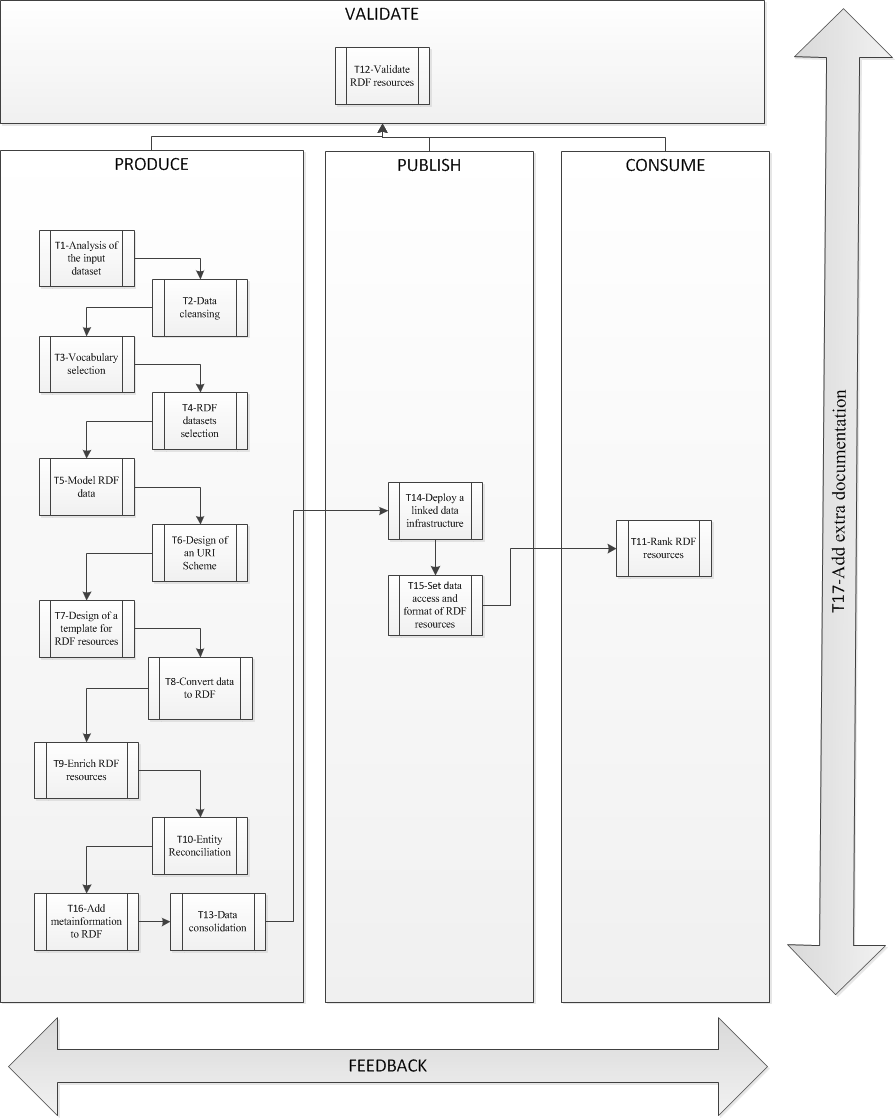
\includegraphics[width=\textwidth]{./imgs/fig-1}
 \caption{Summary of tasks of the MOLDEAS Linked Data lifecycle.}
 \label{fig:summary-tasks}
\end{figure}





  \subsection{Knowledge Organization System Conversion Methods}\label{sect:thesauri}
  This section specifically discusses existing methods to convert knowledge organizations systems distinguishing between RDF/OWL 
conversions methods for thesauri and product classification systems.

\begin{itemize}
 \item \textbf{Thesauri Conversion Methods}. A thesaurus is a controlled vocabulary, with equivalent terms explicitly 
 identified and with ambiguous words or phrases (e.g. homographs) made unique. This set of terms also may include broader-narrower 
 or other relationships. Usually they are considered to be the most complex of controlled vocabularies. Thesauri as a KOS 
 system can be converted by means of different procedures. On the one hand, there are methods~\cite{DBLP:conf/jcdl/Soergel05} that propose specific 
 techniques for thesauri conversions into ontology. However the method does not target a specific output format and it considers the 
 hierarchical structure of thesauri as logical is-a relationships. On the other hand, there are some generic methods 
 for thesauri conversions, as the step-wise method defined in~\cite{DBLP:conf/esws/AssemMMS06}. This method selects a common output data model, the 
 SKOS vocabulary, and is comprised of the following sequenced steps: generation of the RDF encoding, error checking and validation 
 and publishing the RDF triples on the Web. In addition, this method has been refined in~\cite{siedl2008} adding three new sub steps 
 for generating the RDF encoding: analyzing the vocabulary, mapping the vocabulary to SKOS properties and classes and building a conversion program. 
 This initial stepwise method can be considered as a previous effort to the aforementioned linked data lifecycles in which all tasks are already defined and these
 steps are embedded as part of the whole lifecycle.
 
 \item \textbf{Product Scheme Classification Conversion Methods.}  Product Scheme Classifications (PSCs) have been developed to 
 organize the marketplace~\cite{Leukel-automating,Leukel-comparative} in distinct vertical sectors that reflect the 
 activity (or some activities) of economy and commerce. They have been built to solve specific problems of 
 interoperability and communication in e-commerce~\cite{Leukel-findings} providing a structural organization 
 of different kind of products collected together by some economic criteria. The aim of a PSC is to be used 
 as a standard~\cite{Leukel-standard} de facto by different agents for information interchange 
 in marketplaces~\cite{FenselOmel2001,FenselDing2001}. Many approaches for product classification systems adaptation to the Semantic Web, 
 like~\cite{Lonsdale:2010:ROL:1743778.1744005}, present methods with the goal to convert them to domain-ontologies. 
 The tree-based structure between product terms is then interpreted as a logical is-a hierarchy. 
 From our point of view and following the discussion in~\cite{Hepp:2007:POR:1256315.1256337,Hepp:2006:SWS:1128590.1128683}, hierarchical 
 links between the elements of each economic sector have not the semantics of subsumption relationships. The next example 
 taken directly from the CPV 2008 shows how the relationship between the element ``Parts and accessories for bicycles'' (34432000-4) 
 and its direct predecessor, ``Bicycles'' (34430000-0), does not seem an is-a relation. In this case, an ontological 
 property for object composition like \texttt{hasPart} would be much better. Moreover, there are further 
 remarks against the idea of using the PSCs as domain-ontologies. It is difficult to assert 
 that the CPV element, ``Bars, rods, wire and profiles used in construction'' (44330000-2), represents 
 any specific product. Rather it should be regarded as a collection of products. 
 To convert correctly this element into a domain ontology concept, it should be considered 
 as equivalent to the union of several concepts (e.g. $Bar \cup Rod \cup Wire \cup Profile$).
 
 Our approach instead will not consider PCSs as domain ontologies, but a specific kind of knowledge organization system. Any PSC is 
 interpreted as a conceptual scheme comprised of conceptual resources. Thus, hierarchical relationships are not 
 considered to be any more logical \texttt{is-a} relations, but \texttt{broader/narrower} ones. 

\end{itemize}

  \subsection{Least Common Multiple of Controlled Vocabularies}\label{sect:least}
  Knowledge organizing systems are used for managing large collections of information objects and efficient information retrieval. 
Existing controlled vocabularies are currently available in several formats: PDF, MSExcel, CSV or XML. However promoting them 
to the Semantic Web is not a merely process of RDF/OWL conversions. Transformations need to fulfill some requirements. Firstly, 
a common RDF/OWL representation is required to ensure: a) the semantic compatibility between different vocabularies,
b) the processing of vocabularies in a standard way and c) the sharing of vocabularies for third-parties adoption. In this sense, 
the W3C vocabulary ``Simple Knowledge Organization System'' (SKOS) has been especially designed to fully support 
both structural and lexical features of knowledge organization systems and must be necessarily used in this context. 
Secondly, although controlled vocabularies have some specific non-shared features, in practice a distinction between them is very hard to draw. 
We have identified a minimum set of common features for them. The data model should be expressive enough to preserve as much as 
possible the original semantics of primary sources for these common features. Thirdly, a generic method is needed to ensure quality 
of data conversions to correct SKOS instances. That is why the MOLDEAS lifecycle has been selected to perform the promotion 
of PSCs to RDF taking into account their aforementioned special features and making special emphasis in the next points:
\begin{enumerate}
 \item \textbf{URI Scheme generation.} Controlled structured vocabularies and conceptual resources are interpreted in SKOS as RDF 
 resources, in particular, instances of \texttt{skos:ConceptScheme} and \texttt{skos:Concept}. Thus they are referenced by 
 means of URIs.  Although namespaces are out of the scope of this analysis, one of the tasks is the generation of 
 the \texttt{rdf:ID}s of \texttt{skos:Concept} and \texttt{skos:ConceptScheme} from the original source's information. 
 Usually controlled vocabularies provide unique identifiers for their terms or concepts as follows:
 \begin{itemize}
  \item Generating new identifiers for the concepts of the vocabulary. This option introduces additional management. 
  A mapping between elements of the original source and identifiers should be maintained for updating purposes.
  \item Using the string of the preferred term. We would like to point out here that multilingual sources introduce a 
  factor of complexity that it is not present in monolingual systems. In multilingual sources, this solution 
  implies selecting a preferred term in a given natural language, thus promoting one language over the others with a 
  possible non-desired political impact. In addition, a control procedure has to be established to ensure URI updating if the source term changes.
  \item Using the identifier code of an element. This solution avoids the problem of selecting one preferred language 
  to encode concept URIs. Moreover, codes are usually strings composed of a serial number 
  (legal URI characters) and it preserves the original semantics of a multilingual resource,
  where these codes identify unique terms or concepts and establish mappings between different languages. 
  This last option has been chosen keeping in mind the desired feature of having ``Cool URIs'' to identify RDF resources.
 \end{itemize}

 \item \textbf{Hierarchy formalization.} From our point of view, one of the common aspects shared by 
 KOS is a hierarchy-based structure, at least by thesauri, taxonomies and by most of 
 classification schemes. Hierarchical relations establish links between conceptual resources, 
 showing that the semantics of a resource is, in some way, more general (``broader'') than other (``narrower''). 
 In SKOS, the properties \texttt{skos:broader} and \texttt{skos:narrower} are only used to assert hierarchical 
 statements between two conceptual resources. By the way, these properties are currently not defined 
 as transitive properties. Nevertheless, third-parties, if they consider valuable, can use an OWL reasoner 
 to infer the transitive closure of the hierarchy by means of using both transitive sub properties 
 \texttt{skos:broaderTransitive} and \texttt{skos:narrowerTransitive}. From a theoretical point of view, the transitive closure of hierarchical relations 
 of KOS is still an open issue. Transitive logical formalizations (e.g. using a Description Logics-based language such as SKOS/OWL) 
 of broader/narrower properties have some risks. Cycles can appear in the hierarchical-based structured 
 of controlled vocabularies. Even though, transitive closure of these properties can be useful for 
 search applications to expand original user-queries with terms hierarchically related. In our conversion-method, 
 we have followed the recommendation of the current SKOS specification.
 
 \item \textbf{Multilingual and lexical features.} Regarding controlled vocabularies, 
 multilinguism is a critical issue, especially in European vocabularies such as the CPV. 
 Thesaurus are accessible in $21$ ($23$) official languages of the European Union 
 (Bulgarian, Spanish, Czech, Danish, German, Estonian, Greek, English, French, Italian, Latvian, Lithuanian, 
 Hungarian, Dutch, Polish, Portuguese, Romanian, Slovak, Slovene, Finnish and Swedish) and others such as Croatian. 
 In SKOS conceptual resources are labeled with any number of lexical strings, in any given natural 
 language identified by the \texttt{xml:lang} attribute, following normative RDF/XML syntax. 
 One of these labels is selected as the \texttt{skos:prefLabel} for any given language, and the 
 others as values of \texttt{skos:altLabel}.
 
\end{enumerate}

  \subsection{Application of the MOLDEAS lifecycle to Product Scheme Classifications}\label{sect:use-moldeas}
  Previous sections have outlined the importance of PSCs to improve the accesibility and other issues in 
the e-Procurement sector. The applicability of semantic technologies and Linked Data has been also presented 
as a method to improve interoperability and integration among systems. Furthermore the MOLDEAS lifecycle has been 
also outlined as well as existing conversion methods and common features of PSCs. In order to carry out 
the promotion of PSCs to Linked Data following this lifecycle, a detailed summary of the main tasks is presented below.

\begin{itemize}
 \item  Firstly, the criteria to select and promote PSCs, see Table~\ref{table:pscs-ld}, are presented:
\begin{itemize}
 \item The use of the CPV 2008 is mandatory for all public procurement notices according 
 to the Regulation (EC) Nº 2195/2002 of the European Parliament and it is used as a hub classification.
 \item European classifications such as CPC or CPA have direct mappings (hand-made) to the CPV so they perfectly fit 
 to the task $t_8$ of interlinking RDF resources (the SKOS property \texttt{skos:exactMatch} can be used for this purpose).
 \item International classifications such as ISIC, SITC or NAICS enable the interoperability with 
 other e-Procurement and e-Commerce systems as well as activities in the field of statistics.
 \item GoodRelations and Product Ontology (PO) are two of the main references in the e-Commerce sector. 
 That is why we reuse their definitions and instances with the objective of aligning the linkage of PSCs to existing efforts. 
 \item Other classifications such as TARIC, UNSPSC, PRODCOM or NAPCS are ongoing work and they will be also linked to the CPV.
\end{itemize}

\begin{table}[!ht]
\renewcommand{\arraystretch}{1.3}
\begin{center}
\begin{tabular}[c]{|p{6cm}|l|p{6cm}|} 
\hline
  \textbf{PSC} &  \textbf{Acronym} & \textbf{Source} \\\hline
  Common Procurement Vocabulary, (2003 and 2008) & CPV & European Union \\ \hline
  Combined Nomenclature 2012 & CN & European Union \\ \hline
  Central Product Classification, version 2 (2008) & CPC & European Union \\ \hline
  Product Classification by Activity (2008) & CPA & European Union \\ \hline
  International Standard Industrial Classification of All Economic Activities, Rev.4 & ISIC & United Nations Statistics Division \\ \hline
  North American Industry Classification System 2007 y 2012 & NAICS & United States \\ \hline
  Standard International Trade Classification, Revision 4 & SITC & United Nations Statistics Division \\ \hline
%\textit{Nomenclature générale des activités économiques dans les Communautés européennes} & NACE & Unión Europea \\ \hline
\hline
\end{tabular}
\caption{Product Scheme Classifications.}\label{table:pscs-ld}
  \end{center}
\end{table} 

 \item Tasks $t_1$ and $t_5$. There is an implicit structure in each product classification 
 that enables the use of graph definitions (tree and forest), see Figure~\ref{fig:pscs-data-model}.
 \begin{itemize}
  \item Product categories. A PSC is divided into product categories, $Cat^k_{psc}$, that group different elements according to 
  hierarchy levels generating a disjointed set of elements. Thus, each PSC element or term is defined in only one $Cat^k_{psc}$.
  \item Taxonomy. Apart from categories and hierarchy division, each product sector can be considered as a tree, $T_{psc}$, 
  and the whole set of trees builds a forest, $F_{psc}$. Each $t^0_{psc}$ element is the root of a product sector, each $t_{psc}$ 
  is part of only one $T_{psc}$ and the set product sectors are also disjointed by the forest definition.
 \end{itemize}
 
 The use of the SKOS Core Recommendation to model PSCs is then justified due to the fact this ontology is based on two 
 main classes \texttt{skos:Concept} and \texttt{skos:ConceptScheme}. Thus all PSC elements are 
 an instance of the class \texttt{skos:Concept}. Therefore the interpreation of each element $t_{psc}$ 
 is obvious and avoids the issues presented in Section~\ref{sect:least} keeping all original PSC semantics. In order 
 to group all PSC elements under a common concept, a new class $PSCConcept$ is defined as subclass of 
 \texttt{skos:Concept}. Furthermore this class can be divided into different categories to represent 
 the conceptual hierarchy of the PSC, if any. Thus for each $Cat_{psc}^k$ a subclass of $PSCConcept$ can be defined, e.g. 
 Equation~\ref{cpv-st} represents the CPV structure.
 
 \begin{equation}\label{cpv-st}
 \begin{split}
 PSCConcept\ \equiv Division\ \sqcup\ Group \sqcup\ Class \sqcup\ Category \\
 Division \sqcap\ Group \sqcap\ Class\ \sqcap\ Category = \perp
 \end{split}
\end{equation}

  As Section~\ref{sect:least} has outlined, the PSC taxonomy should not be interpreted as a classical \texttt{is-a} hierarchy but 
  the SKOS Core ontology defines specific properties such as \texttt{skos:inScheme}, \texttt{skos:related}, \texttt{skos:broader Transitive} or
  \texttt{skos:narrowerTransitive} that perfectly match the requirements of establishing relationships among PSC elements. Finally an 
  instance of a ``semantized'' PSC element, $t_{psc}$, is presented in Table~\ref{table:properties}. 
  
 \begin{figure}[!ht]
\centering
	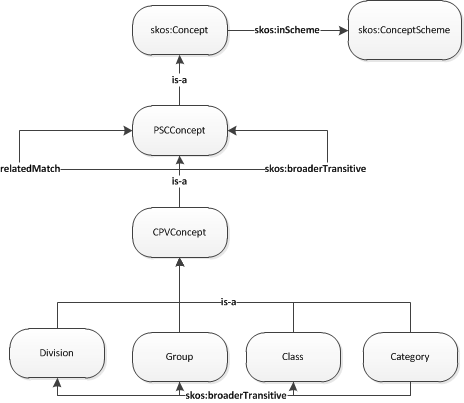
\includegraphics[width=\textwidth]{./imgs/fig-2}
 \caption{A partial view of the data model for PSCs in SKOS.}
 \label{fig:pscs-data-model}
\end{figure}

 \begin{table}[!ht]
\renewcommand{\arraystretch}{1.3}
\begin{center}
\begin{tabular}[c]{|p{3.55cm}|p{5.5cm}|p{5cm}|} 
\hline
  \textbf{Property} &  \textbf{Description} & \textbf{Example} \\\hline
  \texttt{rdf:type} & Type of a PSC element $t_{psc}$ & a \texttt{gr:ProductOr ServiceModel}, \texttt{PSCConcept} \\ \hline
  \texttt{skos:inScheme} & URI to the PSC dataset $T_{psc}$ & \texttt{skos:inScheme} cpv2008:ds \\ \hline
  \texttt{dct:identifier} & Id used in the URI of the element $t_{psc}$ &  \texttt{dc:identifier} "30210000"$\textasciicircum\textasciicircum$xsd:string \\ \hline
  \texttt{dct:subject} & Original Id of the element $t_{psc}$ &  \texttt{dc:subject} "30210000-4"$\textasciicircum\textasciicircum$xsd:string \\ \hline
  \texttt{skos:closeMatch} and \texttt{pscs:relatedMatch} & URI to a target PSC element $t'_{psc}$ that is partially related to a source PSC element $t_{psc}$ & \texttt{po:machine} \\ \hline
  \texttt{skos:exactMatch} & URI to a target PSC element $t'_{psc}$ that is related to a source PSC element $t_{psc}$ & \texttt{cpv2003:30216000} \\ \hline
  \texttt{pscs:level} & Level in the hierarchy of an element $t_{psc}$ when an explicit hierarchy definition is missing & \texttt{pscs:level} ``5'' \\ \hline  
  \texttt{skos:broader Transitive} & URI to a PSC element $t'_{psc}$ ancestor of a broader PSC element $t_{psc}$ & \texttt{skos:broaderTransitive} cpv2008:30200000 \\ \hline
  \texttt{skos:prefLabel} & Multilingual labels and descriptions &  "Data-processing machines (hardware)"@EN \\ \hline
\hline
\end{tabular}
\caption{Main semantic properties used for describing a PSC element.}\label{table:properties} 
  \end{center}
\end{table} 


\item Task $t_3$. The Linked Data community has released a lot of vocabularies to model information and 
knowledge in different domains. One of the keypoints to improve interoperability among sytems 
keeping semantics and, therefore, reasoning capabilities lies in the reuse of these definitions. That is 
why some existing vocabularies have been selected, see Table~\ref{table:vocabs}, to model the PSCs.


 \begin{table}[!ht]
\renewcommand{\arraystretch}{1.3}
\begin{center}
\begin{tabular}[c]{|l|p{8cm}|} 
\hline
  \textbf{Vocabulary prefix} &  \textbf{Description} \\\hline
 dbpedia &  Reuse of DBPedia concepts and properties \\ \hline 
 dc and dct & Dubling Core properties for describing metadata \\ \hline  
 gr & Use of the GoodRelations vocabulary to describe products and services \\\hline 
 po & Use of the ProductOntology vocabulary to create links to existing product and service definitions\\\hline 
 skos & Taxonomy specification and labeling properties \\ \hline
 void & Description of datasets metadata \\\hline
\hline
\end{tabular}
\caption{Main semantic vocabularies selected to model a PSC. These prefixes have been retrieved using the ``Prefix.cc'' service.}\label{table:vocabs} 
  \end{center}
\end{table} 


\item Task $t_6$. In order to get a successful promotion of raw data, the design of a good URI Scheme 
is a key-task~\cite{Heath_Bizer_2011}. Table~\ref{table:pscs-uri} presents the PSCs URI scheme with the aim of addressing the desired features 
of providing ``Cool Uris'', keep the namespaces under our control, etc. and easing the reuse of RDF resources in the ``Web of Data''.
  
 \begin{table}[!ht]
\renewcommand{\arraystretch}{1.3}
\begin{center}
\begin{tabular}[c]{|p{5cm}|p{4.5cm}|p{5cm}|} 
\hline
  \textbf{URI} &  \textbf{Description} & \textbf{Example} \\\hline
  \url{http://purl.org/weso/pscs/} & URI base: <base\_uri> & NA \\ \hline
  \url{<base_uri>/ontology} & Common definitions & \url{<base_uri>/ontology/PSCConcept} \\ \hline
  \url{<base_uri>/resource/ds} & Description of the PSCs Catalogue & \url{<base_uri>/resource/ds} \\ \hline
  \url{<base_uri>/{psc}/{version|year}} & PSC Namespace & \url{<base_uri>/cpv/2008} \\ \hline
  \url{<base_uri>/{psc}/{version|year}/ontology} & Specific definitions & \url{<base_uri>/cpv/2008/ontology} \\ \hline
  \url{<base_uri>/resource/{psc}/{version|year}/{id}} & URI for RDF resources & \url{<base_uri>/cpv/2008/resource/30210000} \\ \hline
  \url{<base_uri>/resource/{psc}/{version|year}/ds} & Description of the PSC dataset  & \url{<base_uri>/cpv/2008/resource/ds} \\ \hline
\hline
\end{tabular}
\caption{Design of an URI Scheme for the PSCs Catalogue.}\label{table:pscs-uri}
  \end{center}
\end{table} 

\item Task $t_8$. The broad aim of this task is to enable the possibility of querying, 
public procurement notices from any PSC. The mappings can be generated following two approaches: 
1) exact mappings created by a domain expert or 2) related, through the execution of a custom entity reconciliation process 
based on NLP techniques. To do so a PSC reconciliation service has been designed using the Apache Lucene and Solr libraries in which
both filters and the syntactic search engine can be easily customized. Firstly a target PSC is selected and their descriptors (in English) 
are indexed using Apache Lucene. After that the mappings between elements in a source PSC are automatically discoverd and generated through the execution 
of queries against the indexed PSC. Basically the creation of a mapping lies in a string comparison between the source descriptor and the 
target descriptor. Nevertheless the personalization of Apache Lucene and Solr allows us the creation of more accurate mappings.

\item Task $t_9$. Since a model for representing PSCs is available the real transformation to RDF has been performed using Google Refine 
and a Java processor. The results of promoting to RDF the selected PSCs are presented in Table~\ref{ganancia-terminos}, 
more specifically the first four columns specify respectively the vocabulary of a PSC ($V_{psc}$), the number of elements 
to be promoted (\#$V_{psc}$), the number of generated RDF triples and the number of links to the CPV 2008. 
Thus we have promoted more than $42035$ product descriptions, generating more than $1842053$ triples and creating $21715$ 
links among them. 

Finally, Figure~\ref{fig:example-cpv-code} shows a partial example of a generated RDF resource in which multilinguism features, 
hierarchy relationships and links can be found. Furthermore, data can be now exploited through SPARQL queries 
such as ``Give me 100 products or services related to construction in any PSC that have a mapping with products or 
services in CPV (descriptions in English)'', see Figure~\ref{fig:example-sparql-query}, using more descriptors and 
different vocabularies.

\item Other tasks such as ``Add metainformation'' are considered optional but relevant to mainly ease the process of dataset discovery.

\item Task $t_{14}$. Once the PSCs are available as RDF is necessary to make them publicly available through a Linked Data infrastructure. To 
do so all RDF triples and the ontology have been deployed in a RDF repository (OpenLink Virtuoso), thus data can be accessed through 
a SPARQL endpoint. Furthermore and with the aim of making dereferenceable URIs and enabling content negotiation an instance 
of Pubby (a Linked Data frontend) has been also deployed. Besides in order to ease the creation and execution of SPARQL queries, SNORQL 
(a tool for exploring SPARQL endpoints) has been also released. Finally, the new PSCs catalogue has been released to the 
LOD community, added to the ``datahub.io'' register and joined the LOD Cloud Diagram under the dataset id ``\texttt{pscs-catalogue}''.

\item Task $t_{12}$. The MOLDEAS lifecycle purposes a validation method based on a checklist of $196$ points compiled from books, 
W3C specifications, Open Data and Linked Data principles, CKAN validator, LOD Cloud requirements, etc. which values can be 
``Applicable and positive (Yes)'', ``Applicable and not found (No)'' or ``Not Applicable (N/A)''. The objective of this questionnaire is 
to ensure the principles of the LOD initiative for easing the reuse, maintenance, governance, coverage and expressivity of data. In order to compare 
the new version of a PSCs catalogue to existing public versions, we have carried out this survey obtaining the next results, 
see Figure~\ref{fig:results-4}, in which ``Reference'' corresponds to the MOLDEAS lifecycle perfect evaluation, ``CSV/Excel'' to the official publicly 
available versions of PCSs and ``Third-parties service'' to those versions managed by non-official organizations. 

 \begin{figure}[!ht]
\centering
	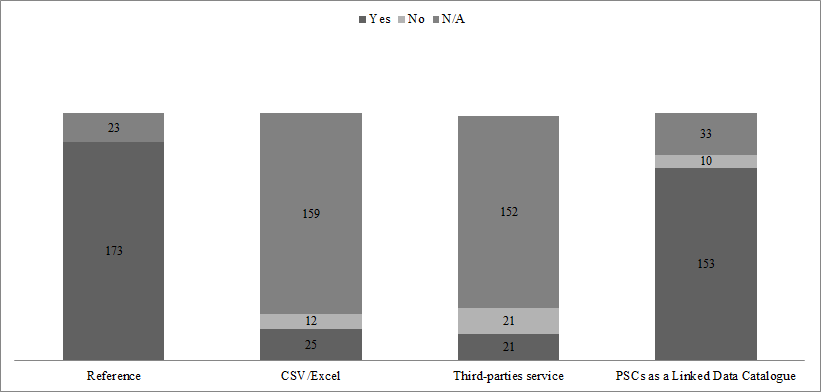
\includegraphics[width=12cm]{./imgs/fig-4}
 \caption{Validation and comparison of the PSCs Catalogue as Linked Data with regards to existing versions.}
 \label{fig:results-4}
\end{figure}



\end{itemize}



\begin{figure}[!ht]
\begin{lstlisting}[language=SQL,basicstyle=\ttfamily\scriptsize]  
cpv2008-res:30210000 a gr:ProductOrServiceModel, cpv-onto:Group;
  skos:prefLabel, gr:description, rdfs:label 	
  "Data-processing machines (hardware)"@EN ,
  "Naprave za obdelavo podatkov (strojna oprema)"@SL , 
  "Databehandlingsmaskiner (hardware)"@DA ,
  "Macchine per l'elaborazione di dati (hardware)"@IT ,
  "Databehandlingsmaskiner (maskinvara)"@SV ,
  "Maşini de procesare a datelor (hardware)"@RO ,   
  "Machines voor dataprocessing (hardware)"@NL , 
  ... ;
  dct:identifier "30210000"^^xsd:string;
  dct:subject "30210000-4"^^xsd:string;
  pscs-onto:relatedMatch   
    <http://www.productontology.org/id/dataprocessing>,
    <http://www.productontology.org/id/hardware> ,
    <http://www.productontology.org/id/machine> ;	
  skos:broaderTransitive cpv2008-res:30200000;
  skos:exactMatch 
    cpv2003-res:30216000, cpv2003-res:30215000,  cpv2003-res:30213000,   
    cpv2003-res:30212000, cpv2003-res:30211000,  cpv2003-res:30214000.
\end{lstlisting}
\caption{Partial example of CPV 2008 item in RDF.}
 \label{fig:example-cpv-code}
\end{figure}


\begin{figure}[!ht]
\begin{lstlisting}[language=SQL,basicstyle=\ttfamily\scriptsize]  
SELECT DISTINCT * WHERE{
   ?product pscs:relatedMatch 
    <http://www.productontology.org/id/construction> .
   ?product skos:closeMatch ?cpv .
   ?product skos:prefLabel ?productLabel .
   ?cpv skos:prefLabel ?cpvLabel .
   ?product skos:inScheme ?scheme .
   FILTER (?scheme != <http://purl.org/weso/pscs/cpv/2008/resource/ds>) .
   FILTER (lang (?cpvLabel) ="en" )
} LIMIT 100
\end{lstlisting}
\caption{Example of SPARQL query.}
 \label{fig:example-sparql-query}
\end{figure}




\clearpage
\section{Evaluation}\label{sect:evaluation}
In order to evaluate if the approach to generate Linked Data from PSCs can improve the access to public procurement data 
exploiting the advantages of this initiative, an evaluation of the number of links and its application to implement a decision 
support system has been carried out. The first studio check if we can access more public procurement notices when the 
links between a PSC and the CPV are created. The aim of this study is to compare the initial input vocabulary (containing the CPV descriptors) and 
the final input vocabulary (containing the descriptors of the PSCs linked to the CPV). If we extend the input vocabulary we can access to more 
public procurement notices because we have a greater number of descriptors to build SPARQL queries going from any PSC to the CPV. 
The second study tries to exploit the semantic relationships between the CPV concepts to build a recommender of CPV codes for business users. 
In order to make a real comparison we have used $11$ user queries and the translation into CPV codes made by the company Euroalert.net 
(the real user query and the descriptions of the CPV codes are skipped in order to keep the privacy of this company and their clients).
\subsection{Study 1}
\subsection{Research Design}
The purpose of this study is to compare the size of the initial input vocabulary for retrieving public procurement notices 
with regards to the final input vocabulary when links between a PSC and the CPV are created. The exploitation of these links can be used 
to build new SPARQL queries that can take advantage of Linked Data principles to provide a greater input vocabulary. Let's assume the following points about the 
public procurement notices and the PSCs used in this study:
\begin{itemize}
 \item All public procurement notices are annotated by, at least, one CPV element.
 \item Each PSC is a controlled vocabulary comprised of a finite set of elements. The CPV is a controlled vocabulary, $\mathcal{V}$, comprised of $10357$ elements/terms/codes.
 \item The public procurement notices is a dataset, $\mathcal{D}$, comprised of 1M of documents, 
 already available as RDF resources. Each document, $d \in \mathcal{D}$ is tagged, at least, using a CPV code, $v \in \mathcal{V}$. Thus, 
 if a query contains all elements, $v \in \mathcal{V}$, the entire dataset of notices will be retrieved.
\end{itemize}
Once these assumptions are defined, the gain of linking a new finite PSC to CPV can be calculated as follows:
\begin{itemize}
 \item The source controlled vocabulary, $\mathcal{V}_{psc}$, is comprised of \#$\mathcal{V}_{psc}$ elements.
 \item The linking of terms between a source vocabulary, $\mathcal{V}_{psc}$, and  a target vocabulary, $\mathcal{V}$ can be carried out in the next ways:
 \begin{enumerate}
  \item $1-1$ link, there are elements $v^k_{psc} \in \mathcal{V}_{psc}$ that are linked to only one element $v \in \mathcal{V}$.
  \item $1-n$ link, there are elements $v^k_{psc} \in \mathcal{V}_{psc}$ that are linked to some elements $v \in \mathcal{V}$ generating $K$ links.  
  \item The result of the previous operation generates links or pairs in the form $p_k=(v^k_{psc}, v^k)$ building a set of pairs $\mathcal{P}=\{p_1,p_2,...,p_k,p_n\}$. Taking into account this situation, 
  the initial vocabulary $V$ is increased in all elements $v^k_{psc} \in \mathcal{V}_{psc}$ that have a link to an element $v \in \mathcal{V}$. The new 
  derivate vocabulary $\mathcal{V'}_{psc}$ is a controlled vocabulary comprising all elements $v^k_{psc}: v^k_{psc} \in p_i$.
 \end{enumerate}
 
 \item The percentage of gain in terms of expressivity (number of elements to be used in queries) is related to the number of elements that enables go from $\mathcal{V}_{psc}$ to $\mathcal{V}$:	
 \begin{equation}\label{percentage}
  \%=100*(\frac{\#\mathcal{V'}_{psc} + \#\mathcal{V}}{\#\mathcal{V}}-1)
 \end{equation}
 
  As an example of this approach, two controlled vocabularies and a set of links/pairs are presented to calculate the gain in terms of expressivity:
  \begin{itemize}
  \item Let $\mathcal{V} = \{ 1, 2, 3 \}$  and  $\mathcal{V}_{psc} = \{A, B, C, D, E\}$ the source and target controlled vocabularies.
  \item Let $P = \{ (A,1), (B,2), (C,1) (C,2) \}$ the set of links/pairs between $\mathcal{V}$ and $\mathcal{V}_{psc}$.
  \item Let $\mathcal{V'}_{psc} = \{ A, B, C \}$ the set of elements $v^k_{psc}: v^k_{psc} \in p_i$.
  \item Therefore, the new controlled vocabulary to query the dataset is comprised of $\{\mathcal{V}\,\cup\,\mathcal{V'}_{psc}\}$ and the percentage of gain in terms of expressivity 
  according to the Equation~\ref{percentage} is:

  \begin{equation}
      \% = 100 * \{ \langle (3+3) / 3 \rangle -1 \} = 2-1 = 100 
  \end{equation}
      \item As a consequence the number of final terms to create queries is just two times than the initial set, increasing the expressivity in a $100\%$.
  \end{itemize}

 \item Finally, in this study, there is a specific scenario in which elements $v^k_{psc} \in \mathcal{V}_{psc}$ are not directly mapped to elements $v \in \mathcal{V}$ but 
 assuming that there are relations $r_k$  among elements $v^j_{psc}$  and $v^k_{psc}$ new links could emerge between $v^j_{psc}$ and $v$ through $r_k$. Nevertheless this 
 situation should be avoided in order to prevent an infinite and recursive linking process and keep the advantages of using finite controlled vocabularies, 
 e.g. in the ongoing example, Product Ontology (PO) is used as a bridge classification implying an infinite max gain ($\infty$).
 
\end{itemize}

\subsection{Sample}
The PSCs that have been selected to be promoted to RDF, see Table~\ref{}, are also used to check if the gain we can get through a direct link to the CPV 2008 or 
by means of creating a un-directed link through the ProductOntology.

 

\subsection{Results and Discussion}
Table~\ref{ganancia-terminos} presents the statistics of transforming each PSC as well as the number of terms that have linked to CPV 2008 and the gain (percentage) of 
new descriptors we can use to query the dataset. As an example, the CPV 2008 is comprised of $8323$ elements that have generated $546135$ RDF triples. 
Once this PSC is in RDF, the linking process has created $462$ links between the CPV 2003 and CPV 2008 obtaining a $\% = 100 * \{ \langle (462+10357) / 10357 \rangle -1 \} = 1.0446-1 = 4.46$\% more 
of expressivity (in terms of descriptors to query a dataset) with regards to the initial set of $10357$ terms in CPV 2008. In case of using the ProductOntology as a bridget 
between the CPV 2003 and CPV 2008, $8312$ descriptions in CPV 2003 have linked to the ProductOntology generating a new controlled vocabulary with a 
gain of $80.25$\# in terms of expressivity (it is possible to use...)FIXME: Explain how this value is generated


\begin{table}[!htb]
\renewcommand{\arraystretch}{1.3}
\begin{center}
\begin{tabular}[c]{|p{2.2cm}|p{1.6cm}|p{1.8cm}|p{1.6cm}|p{1.6cm}|p{1.8cm}|p{1.6cm}|}
 
 \hline
  $\mathcal{V}_{psc}$ & $\#\mathcal{V}_{psc}$  & RDF triples &Links to CPV 2008 &  $\%$ real & Links through PO & $\%$ real trough PO    \\\hline

CPV 2008 	& $10357$  	& $803311$	& $0$	 	& $0$	 	& $10000$	& $96,55$	  \\ \hline
CPV 2003 	& $8323$  	& $546135$	& $462$ 	& $4.46$ 	& $8312$	& $80.25$	 \\ \hline
CN 2012  	& $14552$	& $137484$	& $2390$ 	& $23.08$	& $2390$	& $23.08$	  \\ \hline
CPC 2008 	& $4408$	& $100819$   	& $4402$	& $42.50$	& $4403$	& $42.51$ 	  \\ \hline
CPA 2008 	& $5429$	& $92749$   	& $5399$	& $52.13$	& $5410$	& $52.24$	  \\ \hline
ISIC v4  	& $766$		& $18986$   	& $765$ 	& $7.39$ 	& $765$		& $7.39$	   \\ \hline
NAICS 2007 	& $2328$	& $36292$ 	& $2300$	& $22.21$	& $2300$	& $22.21$	 \\ \hline
NAICS 2012 	& $2212$	& $70887$ 	& $2186$	& $21.11$	& $2186$	& $21.11$	  \\ \hline
SITC v4 	& $4017$	& $3811$   	& $3811$	& $36.80$	& $3820$	& $36.88$	 \\ \hline
\multicolumn{7}{|c|}{\textbf{Total}} \\ \hline
$\star$ 	& $42035$ 	& $1842053$	& $21715$   	& $209.66$	& $29586$ 	& $285.66$	 \\ \hline
\hline
%  \multicolumn{7}{|c|}{\textbf{Linking CPV 2008 and \textit{ProductOntology}}} \\ \hline
%  \textit{PO}& $\infty$	& $10000$   	& N/A	& $96.55$					& $96.55$ 	& $\infty$  \\ \hline
% \multicolumn{8}{|c|}{\textbf{Total including \textit{ProductOntology}}} \\ \hline
% $\star$	 & $\infty$	& $31715$   	& $209.66$	& $306.21$	& $39586$ & $382.21$	& $\infty$ \\ \hline
  \end{tabular}
  \caption{Statistics of promoting to RDF selected PSCs and linking them to the CPV 2008.}\label{ganancia-terminos}  
  
  \end{center}
\end{table}



Additionally, the lifecycle applied to promote and validate the data generated from public procurements notices is based on 
a checklist~\cite{} created by a compilation of $196$ checkpoints which a value can be ``Applicable and positive (Yes)'', ``Applicable and not found (No)'' or ``Not Applicable (N/A)''; 
from books, W3C specifications, Open Data and Linked Data principles, CKAN validator, LOD Cloud requirements, etc., 
and know-how acquired in previous projects that seeks for ensuring the principles of the LOD initiative, 
easing the reuse, maintenance, governance, coverage and expressivity of data. 
In order to compare the new version of a PSCs catalogue to existing public versions of these classifications, 
we have carried out this survey obtaining the next results, see Figure . Finally, this PSCs catalogue has been released to the LOD community, added to the ``datahub.io'' 
register and joined the LOD Cloud Diagram under the dataset id ``\texttt{pscs-catalogue}''.


\subsection{Study 2}
The aim of this study is to verify if the Linked Data coming from public procurement notices, PSCs, etc. can be consumed to deliver a decision support system that help expert 
users to select CPV codes from user queries in natural language. This study is motivated by the company Euroaler.net that sells an alert service for users (companies, etc.) 
that want to tender in specific sectors under a certain profile. Usually, the most relevant variables in public procurement notices are the CPV codes and the 
location (NUTS codes). In this experiment we simulate the behavior of Euroalert.net employees when they have to translate user queries into CPV codes 
for creating a new alert. Basically, the experiment is based on traditional semantic search and concept query expansion methods that we have designed to 
tackle the recommendation of CPV codes, see. Table~\ref{methods-recommending} and Figure . 
\subsection{Research Design}


\begin{table}[!htb]
\renewcommand{\arraystretch}{1.3}
\begin{center}
\begin{tabular}[c]{|l|p{8.5cm}|p{4.5cm}|} 
\hline
\textbf{Method} &  \textbf{Description} &  \textbf{Technology} \\\hline
$M^1$ & CPV English descriptions are indexed and a syntactic search process is performed for each $Q_i$ & Apache Lucene y Solr \\ \hline
$M^2$ & CPV codes are selected according to the SKOS taxonomy. Previously, the method $M^1$ is applied to extract CPV codes from natural language & $M^1$ + ranking broader/narrower \\ \hline
$M^3$ & Similar to $M^2$ but codes are selected using \textit{Spreading Activation}& $M^1$ + ONTOSPREAD \\ \hline
$M^4$ & Similar to $M^2$ but codes are selected using the analysis of historical relationships in previous public procurement notices & $M^1$ + Apache Mahout \\ \hline
 \end{tabular}
  \caption{Methods for recommending CPV 2008 codes.}\label{methods-recommending}  
    \end{center}
\end{table}


\subsection{Sample}
In order to carry out this study we have used the next samples of data:
\begin{itemize}
\item A dataset of 1 million of public procurement notices provided by Euroalert.net containing CPV and NUTS codes.
\item A set of 11 user queries and the expected CPV codes created by Euroalert.net employees, see Table~\ref{expected-codes} (queries have been ``normalized'' according to one CPV descriptor to keep privacy) .
\item The CPV dataset as Linked Data.
\end{itemize}



\begin{table}[!htb]
\renewcommand{\arraystretch}{1.3}
\begin{center}
\begin{tabular}[c]{|l|p{8.5cm}|p{4cm}|} 
\hline
  \multirow{2}{*}\textbf{$Q_{i}$} &  \textbf{User query-$Q_{str}$} &  \textbf{Number of expected CPV codes-$\#Q^{i}_{cpv}$} \\\hline
  $Q_1$ & ``Comprehensive overview over all environmental technologies renewable energy products'' & $463$ \\ \hline
  $Q_2$ & ``Tendering of public works: housing, hospitals, roads, housing developments, station drinking water treatment, reforestation'' & $35$ \\ \hline
  $Q_3$ & ``Prefabricated buildings'' & $7$ \\ \hline
  $Q_4$ & ``Games for children (parks swings, slides, land of play equipment in the public sphere'' & $26$ \\ \hline
  $Q_5$ & ``Vital signs monitor'' &  $277$\\ \hline
  $Q_6$ & ``Museum and exhibition and product launch services'' & $1$ \\ \hline
  $Q_7$ & ``Voltmeters, instruments measuring electrical quantities, Ammeters, Instruments for checking physical characteristics, hygrometers, thermometers, measuring equipment and control, leak detector, Analyzers, 
  Cable Splicing insulated cable joints kits, screwdrivers, hand tools , screwdriver'' & $117$ \\ \hline
  $Q_8$ & ``Conservation Maintenance of pavements for roads, airfields, bridges, tunnels'' & $13$ \\ \hline
  $Q_9$ & ``Wood poles, Wooden sleepers , Lattice towers'' & $10$ \\ \hline
  $Q_{10}$ & ``Architectural, construction, engineering and inspection services'' &  $173$\\ \hline
  $Q_{11}$ & ``Medical practice and related services'' &  $13$\\ \hline
 \end{tabular}
  \caption{User queries and number of expected CPV codes.}\label{expected-codes}  
    \end{center}
\end{table}




\subsection{Results and Discussion}
According to the results in Table~\ref{table:queries-ir-results}, the method that better match the behavior of an expert user is $M^1$ followed by $M^3$. 
This implies that a method based on natural language processing techniques is the most appropriate to translate user queries into CPV codes. 
Oddly, the results of semantic-based methods, $M^2$ and $M^3$, do not get a good performance. Likely, the type of translation 
that the expert user does is more close to a direct language translation than a real thinking about the 
relationships in the taxonomy. Finally, the exploitation of the historical statistics using Apache Mahout algorithms 
(after different iterations and tests we have chosen the best one based on collaborative filtering) do not seem to reflect 
the expert user behavior. Although search and recommendation should not be compared it is strange than a dataset containing the use 
CPV codes in $1$ million public procurement notices could not improve the traditional syntactic search. Nevertheless, there is an 
open issue that lies in the number of true negative codes that in a second step should be validated by experts. 
Thus, the semantic-based methods could improve their results with regards to the traditional one. 



\begin{table}[!htb]
\renewcommand{\arraystretch}{1.3}
\begin{center}
\scriptsize
\begin{tabular}{|c||c|c|c||c|c|c||c|c|c||c|c|c|}
\hline
 \textbf{$Q_i$}&\multicolumn{3}{|c||}{$M^{1}$} & \multicolumn{3}{|c||}{$M^{2}$}& \multicolumn{3}{|c||}{$M^{3}$} & \multicolumn{3}{|c|}{$M^{4}$} \\ \hline
	  &\textbf{P} & \textbf{R} & \textbf{F1} & \textbf{P} & \textbf{R} & \textbf{F1} & \textbf{P} & \textbf{R} & \textbf{F1} & \textbf{P} & \textbf{R} & \textbf{F1}  \\ \hline \hline
$Q_1$  	  &$0.15$ & $0.08$ & $0.08$ &		$0.15$ & $0.15$ & $0.92$ &	$0.12$ & $0.06$ & $0.94$ &	$0.06$ & $0.06$ & $0.81$ \\ \hline
$Q_2$  	  &$0.09$ & $0.09$ & $0.08$ & 		$0.06$ & $0.06$ & $0.99$ & 	$0.03$ & $0.03$ & $0.99$ & 	$0.03$ & $0.03$ & $1.00$ \\ \hline
$Q_3$  	  &$0.14$ & $0.14$ & $0.08$ & 		$0.14$ & $0.14$ & $1.00$ & 	$0.14$ & $0.14$ & $1.00$ & 	$0.00$ & $0.00$ & $1.00$ \\ \hline
$Q_4$  	  &$0.19$ & $0.19$ & $0.08$ &		$0.00$ & $0.00$ & $0.99$ & 	$0.12$ & $0.12$ & $1.00$ & 	$0.00$ & $0.00$ & $1.00$ \\ \hline
$Q_5$  	  &$0.12$ & $0.01$ & $0.08$ & 		$0.01$ & $0.01$ & $0.95$ & 	$0.08$ & $0.01$ & $0.97$ & 	$0.03$ & $0.03$ & $0.97$ \\ \hline
$Q_6$  	  &$1.00$ & $1.00$ & $0.08$ & 		$0.00$ & $0.00$ & $1.00$ & 	$1.00$ & $1.00$ & $1.00$ & 	$0.10$ & $0.67$ & $0.98$ \\ \hline
$Q_7$  	  &$0.20$ & $0.20$ & $0.08$ & 		$0.09$ & $0.09$ & $0.98$ & 	$0.15$ & $0.16$ & $0.98$ & 	$0.03$ & $0.03$ & $0.99$ \\ \hline
$Q_8$  	  &$0.08$ & $0.08$ & $0.08$ & 		$0.08$ & $0.08$ & $1.00$ & 	$0.08$ & $0.08$ & $1.00$ & 	$0.00$ & $0.00$ & $1.00$ \\ \hline
$Q_9$  	  &$0.50$ & $0.50$ & $0.08$ & 		$0.00$ & $0.00$ & $1.00$ & 	$0.30$ & $0.38$ & $1.00$ & 	$0.00$ & $0.00$ & $1.00$ \\ \hline
$Q_{10}$  &$0.39$ & $0.39$ & $0.08$ & 		$0.42$ & $0.42$ & $0.98$ & 	$0.34$ & $0.35$ & $0.98$ & 	$0.16$ & $0.16$ & $0.99$ \\ \hline
$Q_{11}$  &$0.23$ & $0.23$ & $0.08$ & 		$0.23$ & $0.23$ & $1.00$ & 	$0.15$ & $0.17$ & $1.00$ & 	$0.00$ & $0.00$ & $1.00$ \\ \hline
\multicolumn{13}{|c|}{\textbf{Average of quanitative measures}} \\ \hline
\textbf{Total}  &$0.28$ & $0.26$ & $0.99$ & 	$0.11$ & $0.11$ & $0.98$ &  	$0.23$ & $0.23$ & $0.99$ &  	$0.03$ & $0.03$ & $0.96$ \\ \hline
\hline
 \end{tabular}
\caption{Quantitative measures (P-precision and R-recall) of methods for recommending CPV codes.}\label{table:queries-ir-results}
  \end{center}
\end{table} 



% \begin{table}[!htb]
% \renewcommand{\arraystretch}{1.3}
% \begin{center}
% \begin{tabular}[c]{|l|c|c|c|} 
% \hline
% \textbf{Method} &  \textbf{Precision} &  \textbf{Recall} & \textbf{F1 score} \\\hline
% $M^1$ & $0.28$ & $0.26$ & $0.26$ \\ \hline
% $M^2$ & $0.11$ & $0.11$ & $0.11$ \\ \hline
% $M^3$ & $0.23$ & $0.23$ & $0.23$ \\ \hline
% $M^4$ & $0.03$ & $0.03$ & $0.03$ \\ \hline
%  \end{tabular}
%   \caption{Quantitative measures (average) of methods for recommending CPV codes.}\label{methods-result}  
%     \end{center}
% \end{table}



\section{Conclusions and Future work}\label{sect:conclusions}
The main advantage of applying Linked Data to PSCs lies in the possibility of enhancing the number of terms to 
build enriched SPARQL queries. Thus, a broader input vocabulary can ease the access to more and newer 
public procurement notices as. In the European e-Procurement context, this work represents 
a step-forward to a new data realm in which public procurement data must be a key-enabler for the next 
data-based economy easing the access to business opportunities to companies, specially SMEs, 
and creating the appropriate environment for a real EU-wide public market. According to the EC, e-Procurement may, 
by its nature, be more compatible or facilitate the use of procurement budgets in support of the 
EU 2020 objectives. Some countries have adopted the recommendations of the EU introducing strategies to encourage SMEs 
participation in the procurement processes but the intended participation of the SMEs is still far from the EU expectations. 
That is why the e-Procurement must take advantage of the LOD initiative to boost and encourage 
the access to public procurement opportunities.

On the other hand, the exploitation of Linked Data to create a decision support system helping users to select CPV codes 
from user queries is still an open issue that must be improved applying more advanced techniques: in-depth analysis of the CPV codes, 
make correlations with other variables, etc. Nevertheless, we have demonstrated that the advantages of promoting public procurement 
data, with special focus on PSCs, can bridge the gap between human readable formats and machine-processable data. Moreover, 
this work is part of the MOLDEAS platform in which the application of Linked Data principles to the e-Procurement sector has a 
broader scope. The PSC reconciliation service has been also applied to the ``PublicSpending.net'' initiative with the aim 
of comparing the public spending around the world. Further steps include the application of the life-cycle (and its refinement) 
to other relevant PSCs such UNSPSC, NACE or TARIC, the improvement of the reconciliation service, the deployment of 
a PSCs portal similar to the ``NCBO BioPortal'' and the reporting of results to: 1) the Office for Official Publications 
of the European Communities; 2) the ``Internal Market and Services Directorate General'' (DG MARKT) and 3) the ``Information
Society and Media Directorate General'' (DG INFSO) of the European Commission. As a final future action, 
this work must be aligned to current research trends such as: 

\begin{itemize}
 \item Ensure data quality~\cite{lodq}, provenance~\cite{DBLP:conf/ipaw/HartigZ10} and trust.
 \item Process large datasets in a cloud computing environment~\cite{DBLP:conf/closer/HausenblasGHC12},
 entity reconciliation or dataset management to name a few
\end{itemize}


\bibliographystyle{plain}
% %\bibliographystyle{unsrt}
% % %\bibliographystyle{acm}
\bibliography{references,linked-data}
 % \renewcommand{\bibname}{References}


\end{document}
